
\begin{comment}
また,IoTサービスを開発しているルナネクサスさんへ聞き取りを行った.
・ルナネクサスさんの説明
・ルナネクサスさんが開発しているサービスの説明
・どのような点で困っているのか,等の聞き取り結果
\end{comment}

株式会社ルナネクサスとは,大阪にある組み込み機器メーカーである.
近年のIoTへの注目から,IoTサービスを提供している

株式会社ルナネクサスでは,太陽光発電事業を展開している事業主に対し,発電に係る機器の状態や,発電量等を可視化できるサービスを展開している.
独自に開発したIoT機器を発電に係る機器に取り付け,SORACOM Airというインターネット接続サービスを使用して,機器からの情報をサーバーへ蓄積し,ユーザーへ提供している.
SORACOM Airとは,後術するIoT機器向けのインターネット接続サービスの事である.
図\ref{fig:lunafig}は株式会社ルナネクサスのIoTサービスイメージである.
\begin{figure}[htbp]
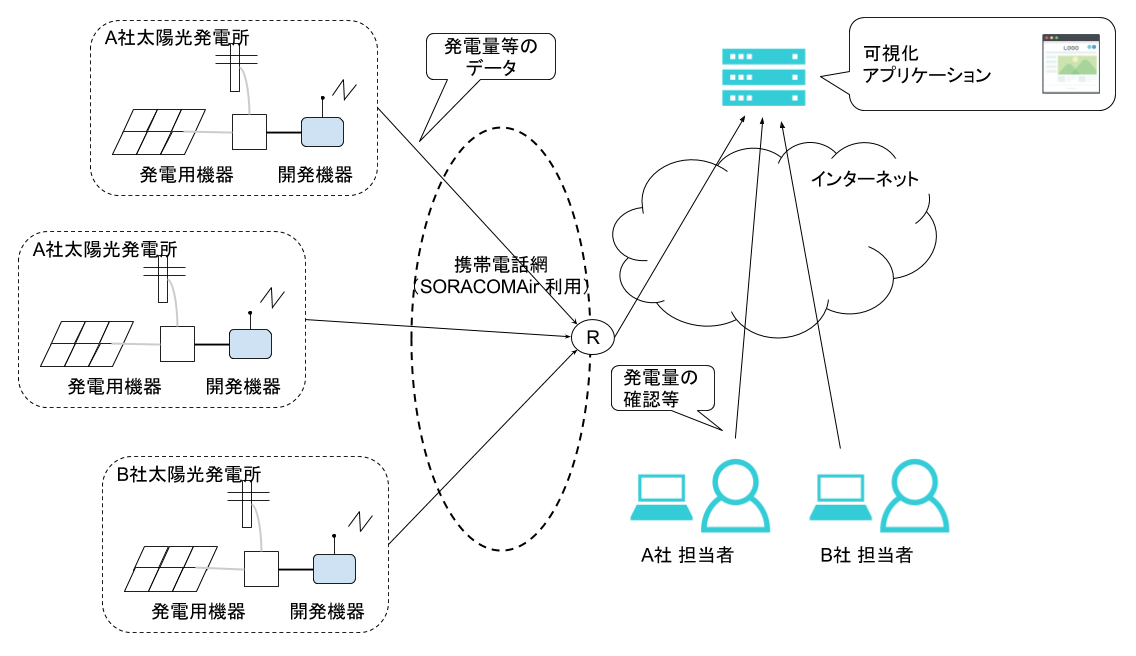
\includegraphics[width=16cm]{images/lunafig.png}
\caption{株式会社ルナネクサス サービスイメージ図}
\label{fig:lunafig}
\end{figure}



太陽光発電に係る機器は,通常発電所のわきに小さなプレハブを建て,その中に設置する.
太陽光発電所は日当たりが良いため,夏場,プレハブの中は太陽の熱と機器が発する熱で機器の標準的な動作温度を超えることがある.
そのため,機器が正常に動作しているかどうかを監視する必要がある.

太陽光発電所は僻地にあることが多いので,利用できるネットワークが無いことが多い.
このことから,インターネットへの接続にSORACOM Airを選択した.
しかし,SORACOMAir回線は,プライベートアドレスを使用しており,IoT機器からの通信は通過するものの,インターネット側からPingなどによる確認を行うことが出来ない.
また,ソフトウェアの更新の為に,ログインするには,現地に行かなくてはならなかった.

この,機器の状態の監視が必要である問題と,遠隔からログインする必要がある問題について,ログインの為にVPNを利用したが,
機器の監視については未解決である.

機器の監視について,どのような事を満たしている必要があるかインタビューを実施した所,以下のような回答をいただくことができた.
\begin{itemize}
\item 単純に機器が起動し,動作している事が確認できれば良い
\item 欲を言うと,CPUの温度等も確認できれば良い
\item 各機器に対するVPNや監視の為の設定も簡略化できたら尚良い
\end{itemize}

\begin{comment}
開発者の役に立つとは,どういうことなのか,

色々と制約があるが,簡単な監視ならできるのではないか,と思い試してみました.
本当はもう何回もやってみて,よりよいものにスべきところなのですが,
\end{comment}

